\section{Mehrere Tabellen abfragen: SQL}
Häufig kann es nützlich sein, mehrere Tabellen miteinander zu verbinden, um neue Einsichten in die Daten zu gewinnen. Verschiedene Tabellen-Verbindungen sind schematisch in \cref{fig:venn-joins} abgebildet. Die Bedeutung dieser Abbildungen wird in den folgenden Abschnitten erklärt.


\begin{figure}[htbp]
\centering

% INNER JOIN
\begin{subfigure}[b]{0.45\textwidth}
    \centering
    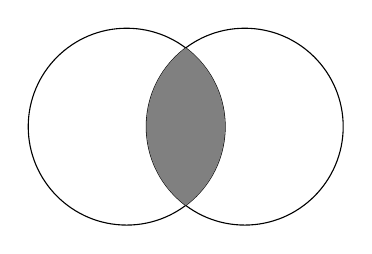
\begin{tikzpicture}
        \tikzset{circle node/.style={circle,draw=black, fill=none, minimum size=25mm, inner sep=0pt}}
        \node[circle node] (left) at (0,0) {};
        \node[circle node] (right) at (1.5,0) {};
        \begin{scope}
            \clip (0,0) circle (1.25cm);
            \fill[gray] (1.5,0) circle (1.25cm);
        \end{scope}
    \end{tikzpicture}
    \caption{\lstinline[style=sql]|INNER JOIN|}
\end{subfigure}
\hfill
% LEFT OUTER JOIN
\begin{subfigure}[b]{0.45\textwidth}
    \centering
    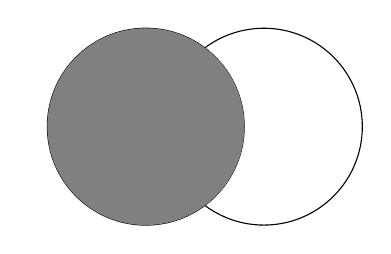
\begin{tikzpicture}
        \tikzset{circle node/.style={circle,draw=black, fill=none, minimum size=25mm, inner sep=0pt}}
        \node[circle node] (left) at (0,0) {};
        \node[circle node] (right) at (1.5,0) {};
        \begin{scope}
            \clip (-1.5,-1.25) rectangle (1.25,1.25);
            \fill[gray] (0,0) circle (1.25cm);
        \end{scope}
        \begin{scope}
            \clip (0,0) circle (1.25cm);
            \fill[gray] (1.5,0) circle (1.25cm);
        \end{scope}
    \end{tikzpicture}
    \caption{\lstinline[style=sql]|LEFT OUTER JOIN|}
\end{subfigure}

\bigskip

% RIGHT OUTER JOIN
\begin{subfigure}[b]{0.45\textwidth}
    \centering
    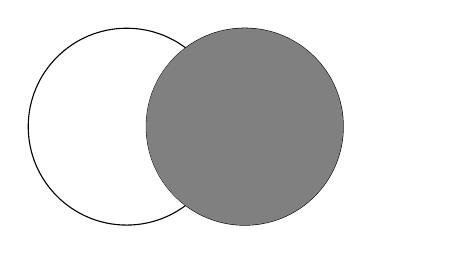
\begin{tikzpicture}
        \tikzset{circle node/.style={circle,draw=black, fill=none, minimum size=25mm, inner sep=0pt}}
        \node[circle node] (left) at (0,0) {};
        \node[circle node] (right) at (1.5,0) {};
        \begin{scope}
            \clip (0,-1.25) rectangle (4,1.25);
            \fill[gray] (1.5,0) circle (1.25cm);
        \end{scope}
        \begin{scope}
            \clip (1.5,0) circle (1.25cm);
            \fill[gray] (0,0) circle (1.25cm);
        \end{scope}
    \end{tikzpicture}
    \caption{\lstinline[style=sql]|RIGHT OUTER JOIN|}
\end{subfigure}
\hfill
% FULL OUTER JOIN
\begin{subfigure}[b]{0.45\textwidth}
    \centering
    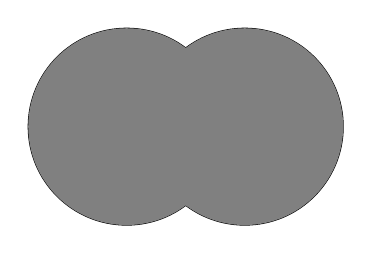
\begin{tikzpicture}
        \tikzset{circle node/.style={circle,draw=black, fill=none, minimum size=25mm, inner sep=0pt}}
        \node[circle node] (left) at (0,0) {};
        \node[circle node] (right) at (1.5,0) {};
        \fill[gray] (0,0) circle (1.25cm);
        \fill[gray] (1.5,0) circle (1.25cm);
    \end{tikzpicture}
    \caption{\lstinline[style=sql]|FULL OUTER JOIN|}
\end{subfigure}
\caption{Venn-Diagramme unterschiedlicher SQL-Joins}
\label{fig:venn-joins}
\end{figure}


\subsection{\lstinline[style=sql]|INNER JOIN| (=\lstinline[style=sql]|JOIN|)}
Die Syntax eines \lstinline[style=sql]|INNER JOIN|-, oder auch einfach \lstinline[style=sql]|JOIN|-Befehls sieht wie folgt aus:

\begin{lstlisting}[style=sql]
SELECT kolonne1, kolonne2, ...
FROM tabelle1
INNER JOIN tabelle2
ON tabelle1.kolonne_id1 = tabelle2.kolonne_id2
\end{lstlisting}
Hier verbinden wir zwei Tabellen, indem wir zwei Kolonnen \texttt{kolonne\_id1} und \texttt{kolonne\_id2}, die derselben Information entsprechen (beispielsweise die user-ID), miteinander abgleichen. Beim \lstinline[style=sql]|INNER JOIN| werden nur die Zeilen aus \texttt{tabelle1} retourniert, für die es einen entsprechenden Wert in \texttt{kolonne\_id2} in \texttt{tabelle2} gibt. Alle Werte in \texttt{tabelle1} die mit keinem Wert in \texttt{tabelle2} überschneiden, sowie umgekehrt, tauchen nicht im Resultat auf (s. \cref{fig:venn-join}).

\begin{figure}[H]
    \centering
    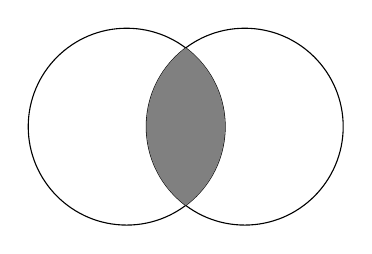
\begin{tikzpicture}
        \tikzset{circle node/.style={circle,draw=black, fill=none, minimum size=25mm, inner sep=0pt}}
        \node[circle node] (left) at (0,0) {};
        \node[circle node] (right) at (1.5,0) {};
        \begin{scope}
            \clip (0,0) circle (1.25cm);
            \fill[gray] (1.5,0) circle (1.25cm);
        \end{scope}
    \end{tikzpicture}
    \caption{\lstinline[style=sql]|(INNER) JOIN|}
    \label{fig:venn-join}
\end{figure}

Wichtig zu wissen ist zudem, dass \texttt{kolonne1, kolonne2} usw. auf der ersten Zeile nun sowohl von \texttt{tabelle1} wie auch \texttt{tabelle2} stammen können.

\begin{myexample}
Folgender Code gibt die ids aller user zurück, denen der user Mika Kaufmann folgt: 
\begin{lstlisting}[style=sql]
SELECT follows.following_id, follows.follower_id, users.name 
FROM follows JOIN users 
ON follows.follower_id = users.id 
WHERE name="Mika Kaufmann"
\end{lstlisting}

Wie Sie sehen, kann es hilfreich sein, im \lstinline[style=sql]|SELECT|-Ausdruck explizit die Tabelle zu nennen, von welcher eine bestimmt Kolonne stammt.

Zudem können auch mehr als zwei Tabellen miteinander verbunden werden.

\end{myexample}

\begin{aufgabe}{}
\begin{itemize}

\item Geben Sie die ids aller Fotos in der Tabelle \texttt{likes} and, die der user Mika Kaufmann gelikt hat.
\begin{myantwort}
\begin{lstlisting}[style=sql]
SELECT photo_id, user_id, name 
FROM likes 
INNER JOIN users 
ON likes.user_id=users.id 
WHERE name="Mika Kaufmann"
\end{lstlisting}
\end{myantwort}
\item Challenge: Erstellen Sie eine Liste, wo für jedes Hamburger Mitglied die Anzahl seiner Fotos aufgeführt ist. Die Liste soll in absteigender Reihenfolge die Anzahl Fotos pro Mitglieder auflisten.
\begin{myantwort}
\begin{lstlisting}[style=sql]
SELECT city, username, COUNT(*) AS "Anzahl Fotos" 
FROM photos 
JOIN users ON photos.user_id = users.id 
WHERE city="Hamburg" 
GROUP BY username 
ORDER BY `Anzahl Fotos` DESC
\end{lstlisting}
\end{myantwort}
\item Es soll Werbung an alle Strandurlauber verschickt werden. Finden Sie alle Photos die den Hashtag \texttt{meer} enthalten. Geben Sie den Namen, die Emailadresse, den Geburtstag und die Stadt der zugehörigen Benutzer aus.
\begin{myantwort}
\begin{lstlisting}[style=sql]
SELECT description, name, email, birthday, city  
FROM photos 
JOIN users on photos.user_id = users.id 
WHERE description LIKE "%#meer%"
\end{lstlisting}
\end{myantwort}
\end{itemize}
\end{aufgabe}

\begin{myabgabe}
Geben Sie die 5 User mit den meisten Followern aus.
\begin{myantwort}
\begin{lstlisting}[style=sql]
SELECT name, COUNT(*) AS "Followers"
FROM users JOIN follows on follows.following_id = users.id 
GROUP BY name
ORDER BY Followers DESC
\end{lstlisting}
\end{myantwort}
\end{myabgabe}

\begin{mychallenge}
Finden Sie heraus, welche 5 Fotos am meisten Likes erhalten haben. Geben Sie den Benutzernamen und Namen der Ersteller der Fotos an, die id der Fotos sowie die Anzahl Likes.
\begin{myantwort}
\begin{lstlisting}[style=sql]
SELECT users.username, users.name AS "Name", photos.id AS "Photo id", COUNT(likes.photo_id) AS "Likes"
FROM users
JOIN photos ON photos.user_id = users.id
JOIN likes ON photos.id = likes.photo_id
GROUP BY users.name, likes.photo_id
ORDER BY Likes DESC
LIMIT 5
\end{lstlisting}
\end{myantwort}

\end{mychallenge}

\subsection{\lstinline[style=sql]|LEFT JOIN| (=\lstinline[style=sql]|LEFT OUTER JOIN|)}
Ein \lstinline[style=sql]|LEFT JOIN|, oder \lstinline[style=sql]|LEFT OUTER JOIN| unterscheidet sich von einem \lstinline[style=sql]|INNER JOIN| dadurch, dass \textbf{alle} Einträge der ersten Tabelle (nach dem \lstinline[style=sql]|SELECT|-Befehl) in der neuen Tabelle erscheinen. Werte aus der zweiten Tabelle, die nicht in der ersten sind, werden jedoch nicht angezeigt (s. \cref{fig:venn-left-join}). 

\begin{figure}[H]
    \centering
    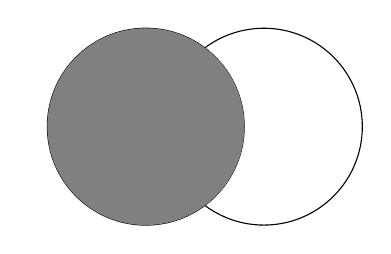
\begin{tikzpicture}
      \tikzset{circle node/.style={circle,draw=black, fill=none, minimum size=25mm, inner sep=0pt}}
        \node[circle node] (left) at (0,0) {};
        \node[circle node] (right) at (1.5,0) {};
        \begin{scope}
            \clip (-1.5,-1.25) rectangle (1.25,1.25);
            \fill[gray] (0,0) circle (1.25cm);
        \end{scope}
        \begin{scope}
            \clip (0,0) circle (1.25cm);
            \fill[gray] (1.5,0) circle (1.25cm);
        \end{scope}
    \end{tikzpicture}
    \caption{\lstinline[style=sql]|LEFT (OUTER) JOIN|}
    \label{fig:venn-left-join}
\end{figure}

\begin{aufgabe}{}
Diejenigen BenutzerInnen, die noch keine Fotos hochgeladen habe, sollen per Email dazu aufgefordert werden, Fotos hochzuladen. Finden Sie alle users, die noch keine Fotos hochgeladen haben. Geben Sie deren Name und Email-Adresse aus. Verwenden Sie statt \lstinline[style=sql]|WHERE| den Befehl \lstinline[style=sql]|HAVING|.
\begin{myantwort}
\begin{lstlisting}[style=sql]
SELECT users.name, users.email, COUNT(photos.id) AS "Anzahl Fotos"
FROM users
LEFT JOIN photos ON photos.user_id = users.id
GROUP BY users.name
HAVING `Anzahl Fotos` = 0
\end{lstlisting}
\end{myantwort}
\end{aufgabe}

\subsection{\lstinline[style=sql]|RIGHT JOIN| (=\lstinline[style=sql]|RIGHT OUTER JOIN|)}
Ein \lstinline[style=sql]|RIGHT JOIN| funktioniert analog zu einem \lstinline[style=sql]|LEFT JOIN| (s. \cref{fig:venn-right-join}).

\begin{figure}[H]
    \centering
    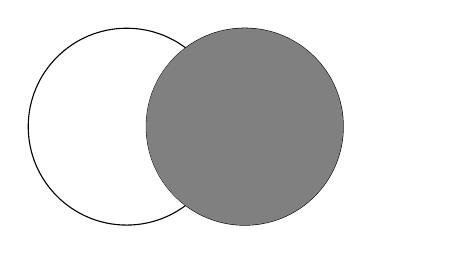
\begin{tikzpicture}
        \tikzset{circle node/.style={circle,draw=black, fill=none, minimum size=25mm, inner sep=0pt}}
        \node[circle node] (left) at (0,0) {};
        \node[circle node] (right) at (1.5,0) {};
        \begin{scope}
            \clip (0,-1.25) rectangle (4,1.25);
            \fill[gray] (1.5,0) circle (1.25cm);
        \end{scope}
        \begin{scope}
            \clip (1.5,0) circle (1.25cm);
            \fill[gray] (0,0) circle (1.25cm);
        \end{scope}
    \end{tikzpicture}
    \caption{\lstinline[style=sql]|RIGHT (OUTER) JOIN|}
    \label{fig:venn-right-join}
\end{figure}


\subsection{\lstinline[style=sql]|FULL JOIN| (=\lstinline[style=sql]|FULL OUTER JOIN|)}
Bei einem \lstinline[style=sql]|FULL (OUTER) JOIN| werden alle Werte aus der ersten und der zweiten Tabelle angezeigt (s. \cref{fig:venn-outer-join}).

\begin{figure}[H]
    \centering
    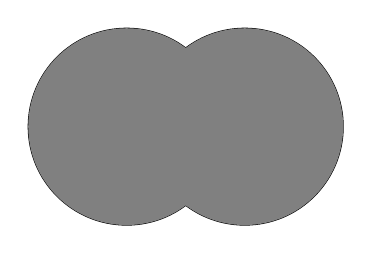
\begin{tikzpicture}
          \tikzset{circle node/.style={circle,draw=black, fill=none, minimum size=25mm, inner sep=0pt}}
                \node[circle node] (left) at (0,0) {};
                \node[circle node] (right) at (1.5,0) {};
                \fill[gray] (0,0) circle (1.25cm);
                \fill[gray] (1.5,0) circle (1.25cm);
    \end{tikzpicture}
    \caption{\lstinline[style=sql]|FULL (OUTER) JOIN|}
    \label{fig:venn-outer-join}
\end{figure}
In InstaHub funktioniert der \lstinline[style=sql]|FULL (OUTER) JOIN| nicht, weshalb es an dieser Stelle keine Übungen hierzu gibt.